\chapter{De regel van Bayes en Markovketens}


\section{Probabiliteit}
\begin{itemize}
	\item Een universum $U$ bevat een eindig aantal toestanden.
	\item De kans op een uitspraak $a$ wordt genoteerd als $p(a)$ en is gelijk aan:
	
	$$p(a) = \frac{\#(a)}{\#U} $$
	met $\#U$ het aantal toestanden in het universum en $\#(a)$ het aantal toestanden waarin $a$ waar is binnen dit universum.
	\begin{itemize}
		\alert Niet bruikbaar: het systeem kan enkel de kans bepalen van reeds bestaande gevallen. 
		\begin{enumerate}
			\item \begin{itemize}
				\item Stel een observatie: $83$-jarige patiënt met hoofdpijn.
				\item In het universum zit er geen $83$-jarige patiënt met hoofdpijn.
				\item De patiënt kan dus niet bestaan.
			\end{itemize}
			\item \begin{itemize}
				\item Stel $43$-jarige patiënt die niet rookt en metselaar is.
				\item In het universum zit één metselaar die $43$ jaar is, niet rookte en psoriasis heeft. 
				\item De patiënt heeft dus psoriasis.
			\end{itemize}
		\end{enumerate}
		
	\end{itemize}
	\item Er is een \textbf{zinvolle veralgemening} nodig.
	\item Het lerend programma moet een \textbf{model} gebruiken waarbij een aantal parameters moet worden ingevuld. 
	\item De waarden van de parameters van dit model kan een zinnige veralgemening geven van probailiteit, via \textbf{de regel van Bayes}.
		
\end{itemize}


\section{De regel van Bayes}
\begin{figure}[t]
	\centering
	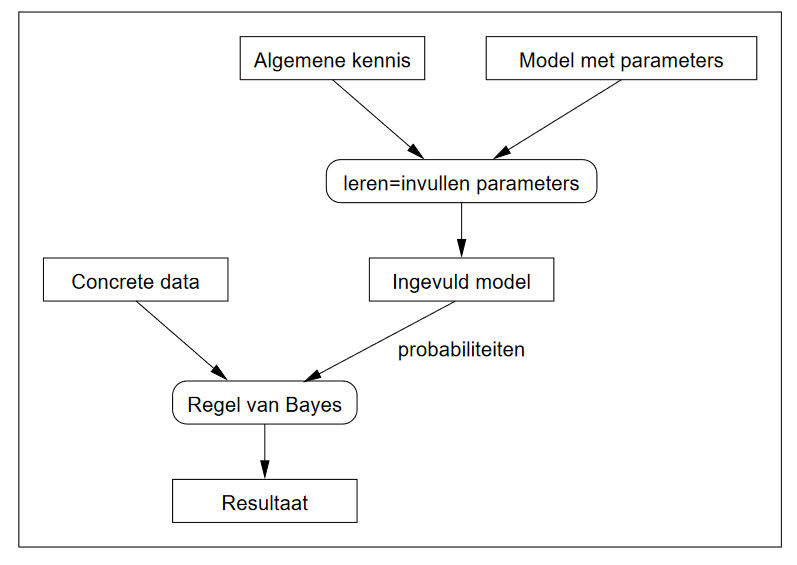
\includegraphics[width=\textwidth]{de_regel_van_bayes}
	\caption{De regel van Bayes bij artificiële intelligentie.}
\end{figure}
\begin{itemize}
	\item De voorwaardelijke kans $p(a|b)$ is de kans dat $a$ waar is gegeven dat $b$ waar is.
	\item Stel $\#U$ het aantal toestanden in het universum en $\#(a)$ het aantal toestanden waarin $a$ waar is:
	
	$$p(a) = \frac{\#(a)}{\#U}, \qquad p(a|b) = \frac{p(a\& b)}{p(b)} = \frac{\#(a\& b)}{\#(b)}$$
	
	\item Dit kan herschreven worden:
	$$p(b)p(a|b) = p(a\& b)$$
	
	zodat 
	$$p(a\& b) = p(b \& a)$$
	
	of 
	
	$$p(b)p(a|b) = p(a)p(b|a)$$
	
	\item \underline{Voorbeeld:} 
	\begin{itemize}
		\item Universum = 10.000 vogels
		\item 1.000 van deze vogels zijn raven: $p(raaf) = 0,1$
		\item 2 van deze vogels zijn wit: $p(wit) = 0,0002$
		\item Er is slechts 1 witte raaf: $p(raaf|wit) = 0,5$ en $p(wit|raaf) = 0,001$ 
		
		\item \textbf{Dus:} $p(wit)p(raaf|wit) = p(raaf)p(wit|raaf) = 0,0001$
	\end{itemize}
	\item Dit kan veralgemeend worden met \textbf{de regel van Bayes}:
	
	$$p(a|b) = \frac{p(a)p(b|a)}{p(b)}$$
	
	\item Veronderstel hypothetische uitspraken $h_i, i = 1, 2, ...$.
	\begin{itemize}
		\item Voor een willekeurig item is exact één hypothetische uitspraak waar.
		\item Het resultaat van een aantal metingen op dat item resulteren in een uitspraak $d$.
		\item Wat is de kans dat een hypothese $h_i$ waar is gegeven de data $d$?
		
		$$p(h_i|d) = \frac{p(h_i)p(d|h_i)}{p(d)}$$
	\end{itemize}
	\item \underline{Voorbeeld:}
	\begin{itemize}
		\item Er is een groot aantal ziektes.
		\item Deze leiden tot de lijst van hypothesen, waarbij $h_i$ staat voor de uitspraak "De patiënt heeft het $i-$de ziektepatroon".
		\item Is er een groot aantal mogelijke symptomen.
		\item Bij een patiënt kunnen de symptomen vastgesteld worden, die resulteren in een uitspraak $d$.
		\item Hoe bepalen welk ziektepatroon het meest waarschijnlijk is?
		\begin{itemize}
			\item $p(h_i)$ is de kans dat ziektepatroon $i$ voorkomt in het universum. Dit is verondersteld gekend te zijn.
			\item $p(d|h_i)$ is de kans dat ziektepatroon $i$ de opgegeven symptomen veroorzaakt. Dit is verondersteld gekend te zijn.
			\item $p(d)$ kan berekend worden uit de vorige gegevens, als er verondersteld wordt dat er bij elke patiënt juist één $i$ is waarvoor $h_i$ waar is:
			
			$$p(d) = \sum_i p(h_i\&d) = \sum_i p(h_i)p(d|h_i)$$
			
			\item De expliciete waarde van $p(d)$ is eigenlijk niet nodig aangezien deze onafhankelijk is van $i$. We weten dat $d$ waar is uit de waarnemingen en is dus een constante factor.
		\end{itemize}
	\end{itemize}
	
\end{itemize}
\section{Markovketens en -modellen}
\begin{itemize}
	\item Wordt gebruikt om tijdsafhankelijke processen te modelleren. 
	\item Formele definitie van een \textbf{Markov model}:
	\begin{enumerate}
		\item Een eindige verzameling van \textbf{staten} $S = \{s_1, ..., s_n\}$. Er is een beginstaat $(s_1)$ en een eindstaat $(s_n)$.
		\item Een \textbf{transitiematrix} $T$. Dit is een $n \times n$ matrix die de probabiliteit van een toestand $s_i$ naar een andere toestand $s_j$ bevat.
		\item Een \textbf{uitvoeralfabet} $A = \{a_1, ..., a_{k - 1}\} \cup \{a_k\}$. Hier is $a_k$ het lege symbool.
		\item Een \textbf{uitvoermatrix} $U$. Een $a \times k$ matrix.
	\end{enumerate}
	\item Een Markovketen kent een probabiliteit toe aan elke string van karakters in $A$. 
	\item Een Markovketen produceert een string, maar niet noodzakelijk altijd dezelfde. Het is \textbf{niet-deterministisch}, maar de kans op een bepaalde string kan wel berekent worden.
	\item Op elk ogenblik is de Markovketen in een bepaalde staat. Voor $t = 0$ is dit $s_1$.
	\item De keten activeren levert een functie $i : \mathcal{N} \rightarrow \{1, ..., n\}$ op die voor elk moment $t$ de index van de staat op dat moment geeft. Op een ogenblik $t$ is de staat $s_{i(t)}$.
	\item De probabiliteiten om van één staat naar een andere te gaan worden in $T$ beschreven:
	
	$$T_{kj} = p(i(t + 1) = j|i(t) = k)$$
	
	Voor een willekeurige $k$ geldt (som der kansen):
	
	$$\sum_j T_{kj} = 1$$
	
	\item De probabiliteit is onafhankelijk van de tijd $t$.
	\item De probabiliteit om op tijdstip $t + 1$ een bepaalde staat te bereiken hangt alleen af van de staat op tijdstip $t$.
	\item De uitvoer van een Markovketen wordt geschreven als $a_{j(t)}$. 
	\item Als op tijdstip $t$ de staat $s_i$ is, dan is de waarschijnlijkheid dat $a_j$ de uitvoer is gelijk aan $U_{ij}$.
	\item Er bestaat dus een één-op-één relatie tussen staat en uitvoer. Hieruit volgt $k = n$, $U_{ii} = 1$ en $U_{ij} = 0$ als $i \neq j$.
	\item Bij een \textbf{\gls{ac:hmm}} kan een staat verschillende mogelijke uitvoeren hebben, en kan een uitvoer horen bij verschillende staten.
	
	\item \underline{Voorbeeld:} Een \gls{ac:hmm} toegepast op spraakherkenning.
	\begin{itemize}
		\item Er bestaat een \gls{ac:hmm} op drie niveaus:
		\begin{enumerate}
			\item Voor elk \textit{foneem}. Dit zijn betekenisvolle klankenreeksen die soms met een letter overeenkomen en soms met een lettergroep.
			\item Voor elk \textit{woord}. Een woord is een opeenvolging van fonemen. 
			\item Voor alle mogelijke zinnen samen.
		\end{enumerate}
		\item Een aantal veronderstellingen:
		\begin{itemize}
			\item Sommige woorden kunnen uitgesproken worden met verschillende fonemen. Hier worden deze als verschillende woorden beschouwd.
			\item Homoniemen worden als hetzelfde woord beschouwd: meid, mijd, mijdt, mijt, ...
			\item Hetzelfde foneem kan traag of snel uitgesproken worden. Deze variatie van lengte wordt aangegeven als de probabiliteit om in dezelfde staat te blijven.
		\end{itemize}
		\item Het meest gebruikelijke model maakt gebruik van drie staten: $B$, $M$ en $E$ (Begin, Midden en Eind), gevolgd door een eindstaat $s_4$. Figuur \ref{fig:hmm_voor_t} toont het HMM voor het foneem 't'.
		\begin{figure}
			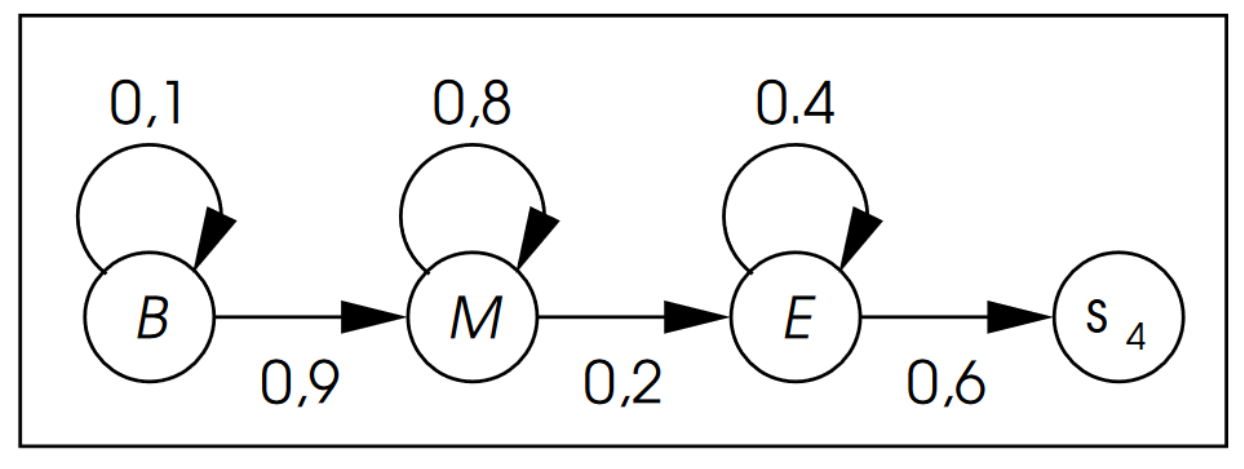
\includegraphics[width=\textwidth]{hmm_voor_t}
			\caption{Het HMM voor het foneem 't'.}
			\label{fig:hmm_voor_t}
		\end{figure}
	
		\item Het HMM voor een woord wordt gevormd door de HMM's voor zijn fonemen aaneen te schakelen. Als een woord $w_i$ de fonemen $f_i$ heeft, dan heeft het HMM 3 $f_i$ staten
		\item Er moet ook nog een model opgebouwd worden om de waarschijnlijkheid van zinnen te modelleren. Dit is echter zeer complex en hierbij wordt er gebruik gemaakt van \textbf{$n$-grammodellen}.
		\begin{itemize}
			\item Een $n$-gram is een sequentie van $n$ woorden.
			\item Als de probabiliteit van alle $n$-grammen gekent is, dan kan dit gebruikt worden om bij $n-1$ woorden het volgende woord te voorspellen.
			\item Een \textbf{unigram} is een $1$-gram dat dan de relatieve frequentie van alle woorden bevat.
			\item Een \textbf{bigram} is een $2$-gram bevat alle mogelijke combinaties van twee opeenvolgende woorden.
		\end{itemize}
		\item Een bigram heeft een beginknoop. Deze beginknoop is verbonden met alle beginknopen van woorden en genereert zelf geen uitvoer. De overgangswaarschijnlijkheid wordt gegeven door de unigrammen. De overgangswaarschijnlijkheid van de eindknoop van een woord naar de beginknoop van een volgend woord is gegeven door de relatieve frequentie van het bijbehorende bigram.
		\item Stel $W$ het aantal woorden en $f$ het gemiddeld aantal fonemen per woord, dan is het totaal aantal staten $3fW$.
	\end{itemize}
	\item In een HMM kan gebruikt worden om de waarschijnlijkheid van een bepaalde uitvoer te berekenen. Maar wat als we willen weten hoe de uitvoer gegenereerd is? 
	\begin{itemize}
		\item 
	\end{itemize}
	
	

\end{itemize}

\section{Leren van het model}
